\documentclass{school-22.101-notes}
\date{November 14, 2011}

\begin{document}
\maketitle




\topic{Semi-Empirical Mass Formula (SEMF): Mass Parabolas, Stability}
Now that we have found the binding energy, we can write an expression for the mass. The mass formula comes out to be \textbf{parabola}, and the minimum mass corresponds to stability\footnote{This is an important point: notice in Eq.~\ref{BAZ}, the smaller the mass, the larger the binding energy, and binding energy is a negative term, so the smaller the total energy, the more stable. }.
\begin{align}
B(A,Z) &= \left[ Z m_H + N m_n - m(A,Z) \right] c^2  \label{BAZ}\\
m(A,Z) c^2 &= \left[ Z m_H + N m_n \right] c^2 - B(A,Z) = Z^2 (\cdots) + Z(\cdots) + C 
\end{align}
That is to say, for a given A, $m(Z)$ is a parabola, then there exists a $Z$ such that $m(Z)$ is minimum, and this is the most stable one. Of course this is a simple approximation that does not take into account stuffs like paring effect yet. 

If we take the derivative of the $m(A,Z)$ equation and set it to zero, we find $Z_{\mathrm{min}}$ to be: 
\eqn{ Z_{\mathrm{min}} \approx \frac{A/2}{1 + \frac{1}{4} \frac{a_c}{a_{\mathrm{sym}}} A^{3/4}} }
At small A, $Z_{\mathrm{min}} \sim \frac{A}{2}$. At large A, $Z_{\mathrm{min}} < \frac{A}{2} \sim 0.41 A$. 

Back to mass parabola, at $Z > Z_{\mathrm{min}}$, there are too many protons; $Z < Z_{\mathrm{min}}$, there are too many neutrons. By nature these nuclei want to undergo decay to reach stability (see Figure~\ref{A135} and Figure~\ref{A102}). 
\begin{enumerate}
\item Proton-rich nuclei go through $\beta^+$ decays: \ce{p^+ \to n + \beta^+ + \gamma}, or Electron Capture (E.C.): \ce{p + e^- \to n + \gamma}. Example: \ce{^{16}_9 F_7 \to ^{16}_8 O_8 + \beta^+ + \gamma}. 
\item Neutron-rich nuclei go through $\beta^-$ decays: \ce{n \to p + \beta^- + \gamma}. Example: \ce{^{16}_7 N_9 \to ^{16}_8 O_8 + \beta^- + \gamma}.
\item For a decay process to happen, it has to be \textcolor{blue}{energetically allowed, $M_{\mathrm{final}} < M_{\mathrm{initial}}$, that is, goes down on the M vs. Z curve.}
\end{enumerate}
\begin{figure}
  \centering
  \subfloat[A=135]{\label{A135}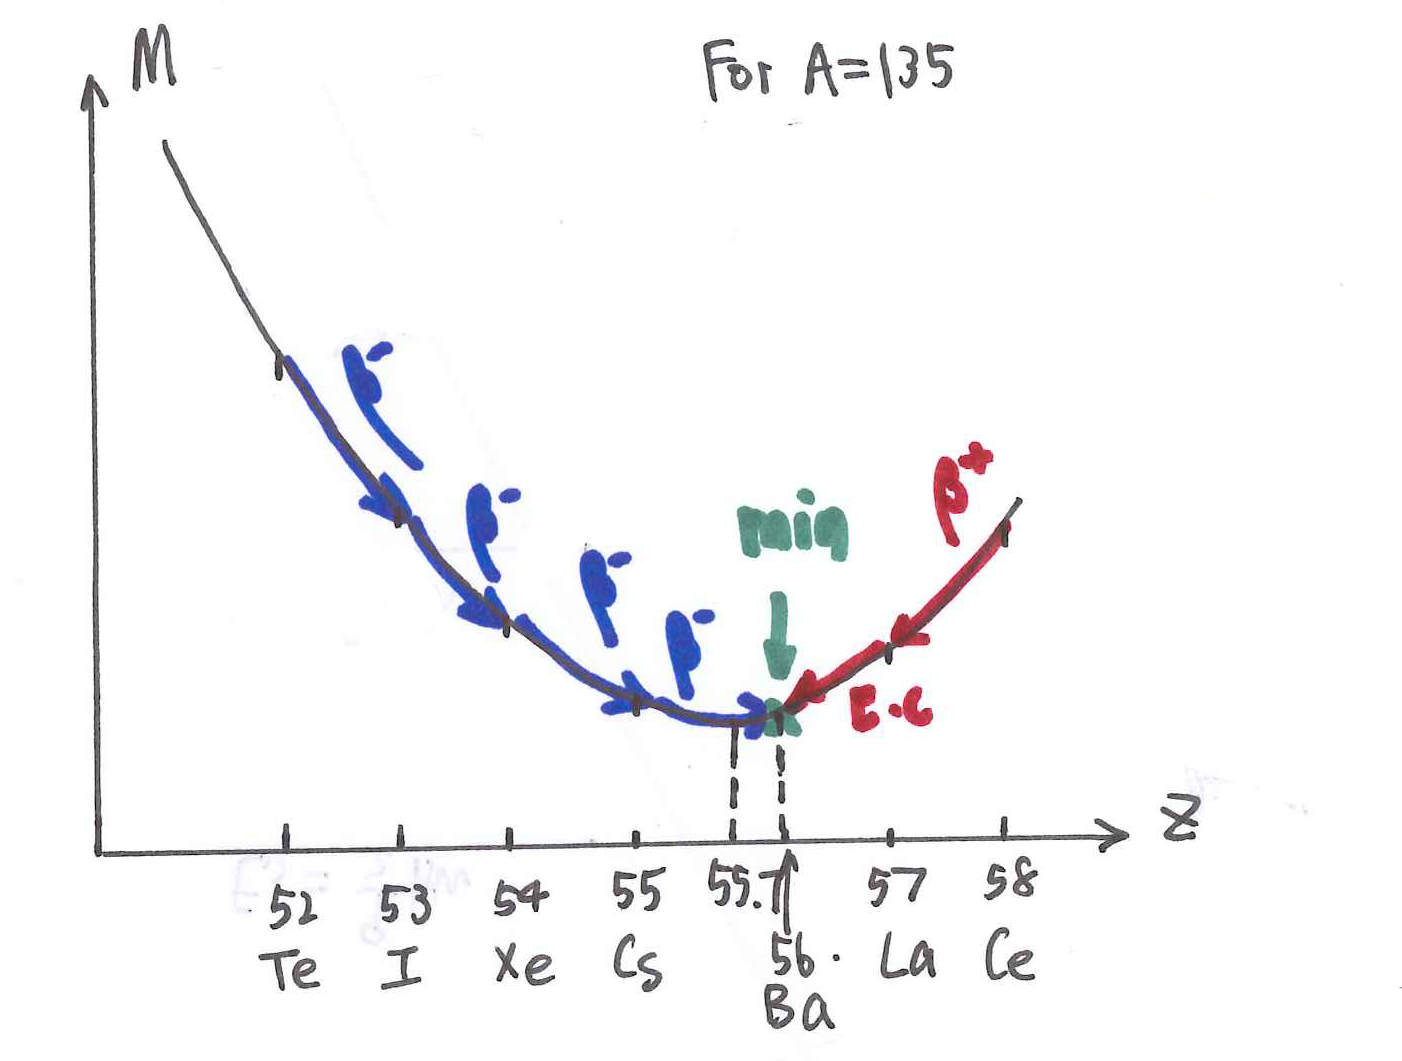
\includegraphics[width=0.4\textwidth]{images/rd/M-Z-A135.png}}                
  \subfloat[A=102]{\label{A102}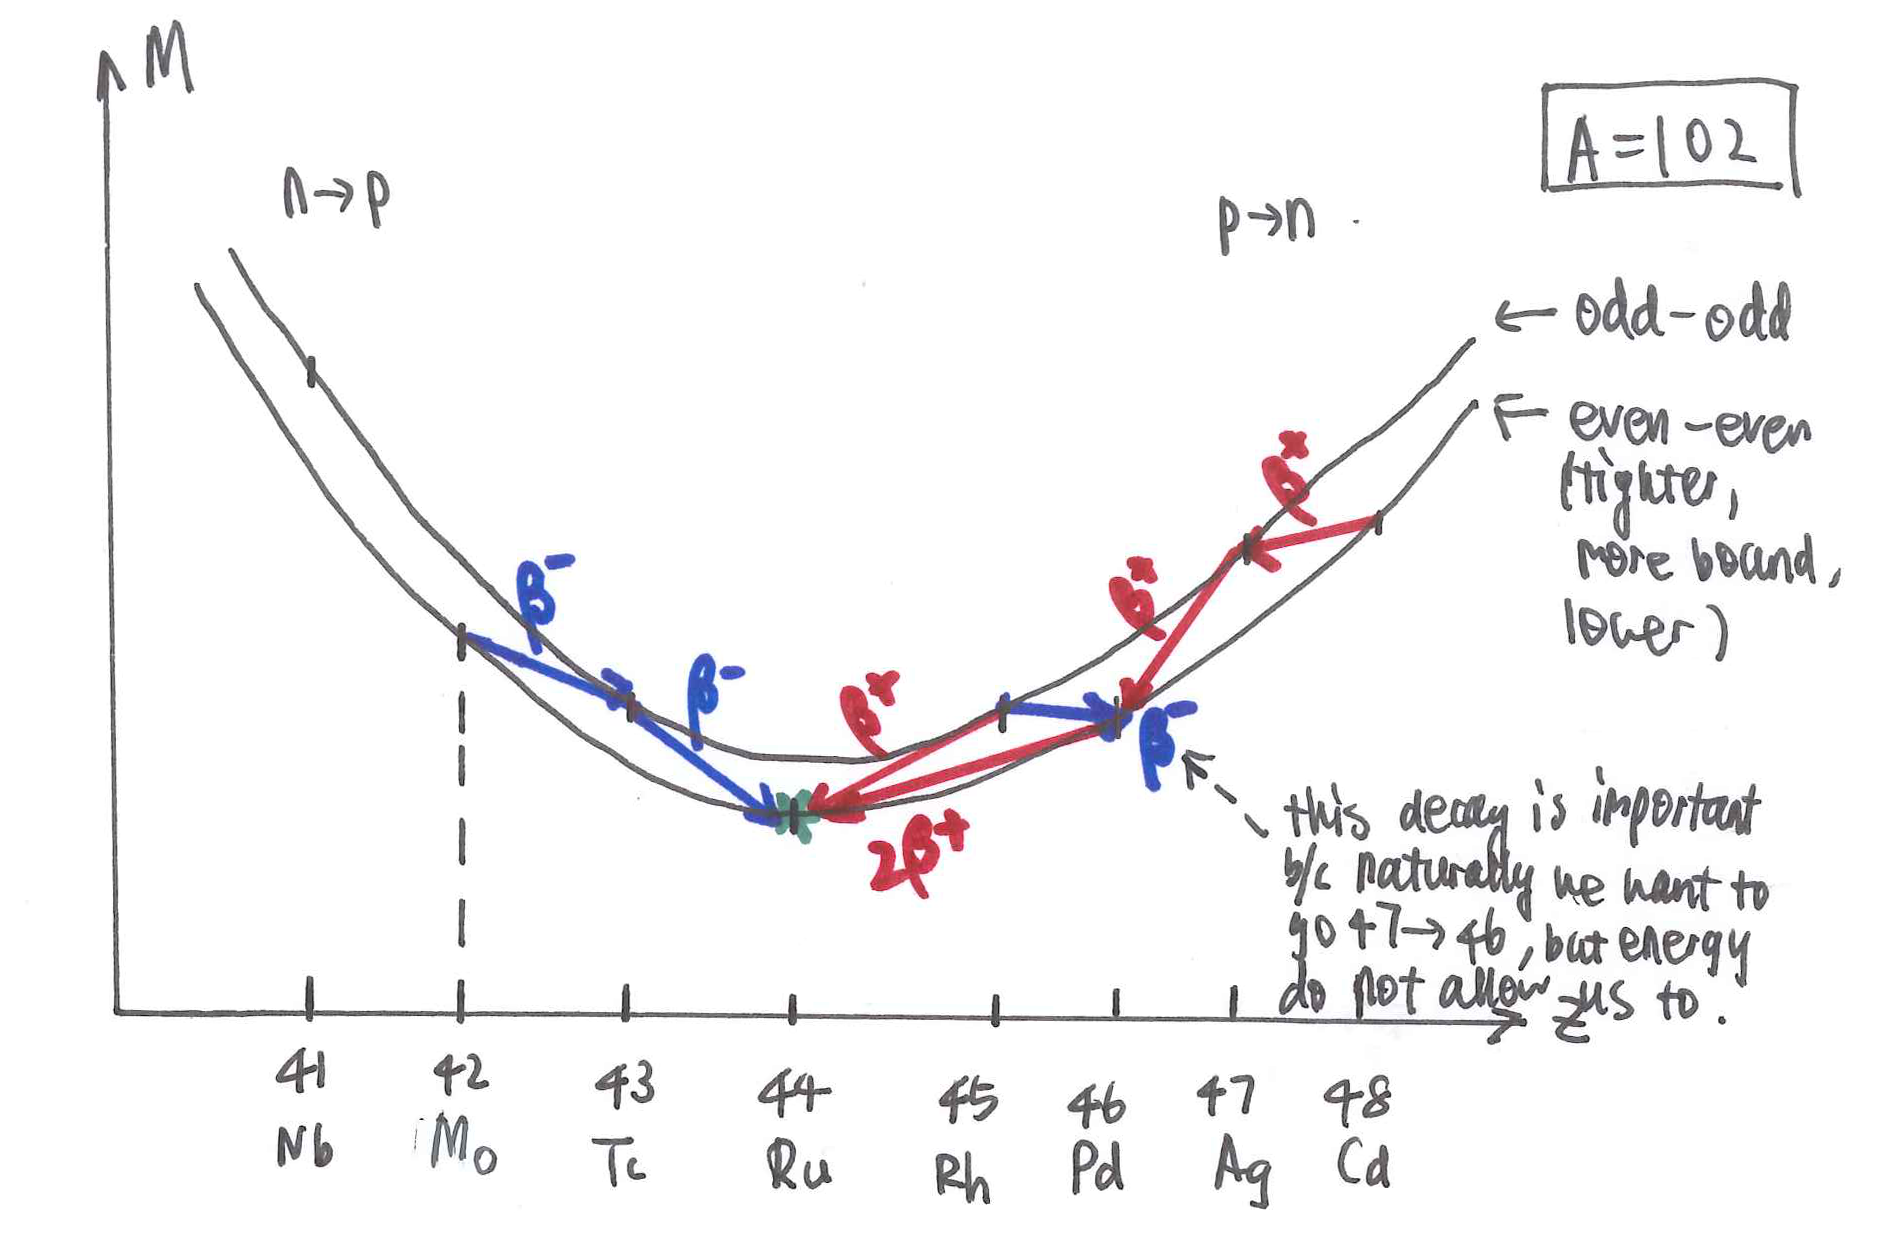
\includegraphics[width=0.6\textwidth]{images/rd/M-Z-A102.png}}
  \caption{Mass Parabola, Two Examples}
\end{figure}
\end{document}
